%
% main.tex -- Paper zum Thema <mongeampere>
%
% (c) 2020 Autor, OST Ostschweizer Fachhochschule
%
% !TEX root = ../../buch.tex
% !TEX encoding = UTF-8
%
\chapter{Monge-Ampèresche Gleichung\label{chapter:mongeampere}}
\kopflinks{Thema}
\begin{refsection}
\chapterauthor{Alain Keller}

Die Monge-Ampèresche Gleichung ist eine Differentialgleichung, welche
im 19 Jahrhundert von Gaspard Monge beschrieben wurde. 
Ihr Ursprüngliches Ziel war es, ein Massentransportprobelm zu lösen. 
% Todo paede kapitel
Im Laufe der Zeit wurden weitere, vor allem mathematische Anwendungen
gefunden.
Eine solche Anwendung in der Differentialgeometrie wird in diesem Kapitel näher 
untersucht.

%
% einleitung.tex -- Beispiel-File für die Einleitung
%
% (c) 2020 Prof Dr Andreas Müller, Hochschule Rapperswil
%
% !TEX root = ../../paper.tex
% !TEX encoding = UTF-8
%
\section{Geschichte\label{geostrophisch:section:teil0}}
\kopfrechts{Geschichte}

Hier folgt nun die Geschichte von Richardson's dream. 

Lewis Fry Richardson war ein britischer Meteorologe und Friedensforscher.
Er berechnete die aller erste numerische Wettervorhersage im Jahre 1922.

\begin{figure}[h]
	\centering
	\includegraphics[width=0.7\textwidth]{LewisFryRichardson.jpg}
	\caption{text}
	\label{bild:portraitRichi}
\end{figure}

Siehe ~\ref{bild:portraitRichi} das ist ein Portrait Foto von Richardson. 



%
% teil1.tex -- Beispiel-File für das Paper
%
% (c) 2020 Prof Dr Andreas Müller, Hochschule Rapperswil
%
% !TEX root = ../../buch.tex
% !TEX encoding = UTF-8
%
\section{Geostrophischer Wind
\label{geostrophisch:section:geoWind}}
\kopfrechts{Problemstellung}


\subsection{Corioliskraft
\label{geostrophisch:subsection:coriolis}}
Die Corioliskraft, welche durch die Rotation der Erde entsteht, beeinflusst die Bewegung von Luftmassen und anderen frei beweglichen Körpern auf der Erdoberfläche. Sie ist eine Scheinkraft, die nur in einem rotierenden Bezugssystem wie dem der Erde auftritt. Die Stärke hängt von der geografischen Breite ab und nimmt in Richtung der Pole zu.
Der Coriolisparameter $f$ beschreibt diese Abhängigkeit und ist definiert als 
\begin{equation}
f\, 
= 
2\Omega\sin(\phi)
\label{geostrophisch:equation1}.
\end{equation}
In dieser Gleichung steht $\Omega$ für die Winkelgeschwindigkeit der Erdrotation und $\phi$ für die geografische Breite auf der Erdoberfläche.
Die Corioliskraft wirkt immer senkrecht zur Bewegungsrichtung. In der Meteorologie betrachtet man sie in der Regel pro Masseneinheit, da sich die Masse eines Luftpakets nicht eindeutig festlegen lässt. Auf der Nordhalbkugel lenkt sie Bewegungen nach rechts ab, auf der Südhalbkugel nach links. Mathematisch lässt sie sich für eine Geschwindigkeit $\vec{v}_g $ mit Hilfe des Kreuzproduktes darstellen. 
Die Corioliskraft pro Masseneinheit ergibt sich wie folgt
\begin{equation}
\frac{\vec{F}_c} {m}
= 
-f\, (\vec{k} \times \vec{v}_g) 
\label{geostrophisch:equation2},
\end{equation}
wobei $\vec{k}$ ein Einheitsvektor in Vertikalrichtung ist.
\begin{equation}
\vec{k} =
\left(
\begin{array}{c}
0 \\
0 \\
1
\end{array}
\right)
\label{geostrophisch:equation3}
\end{equation}
Das Kreuzprodukt von $\vec{k}$ mit  $\vec{v}_g $ sorgt dafür, dass die Corioliskraft immer genau senkrecht zur Bewegungsrichtung wirkt.
\subsection{Gradientenkraft
\label{geostrophisch:subsection:gradient}}
Die Gradientenkraft ist die treibende Kraft pro Masseneinheit, die entsteht, wenn zwischen zwei Orten ein Druckunterschied besteht. Sie wirkt immer von Gebieten mit hohem Druck in Richtung niedrigen Drucks und ist die wichtigste antreibende Kraft für Luftbewegungen in der Atmosphäre. Je größer der Druckunterschied über eine bestimmte Entfernung, desto stärker ist die Gradientenkraft.
Mathematisch lässt sie sich wie folgt beschreiben:
\begin{equation}
\frac{\vec{F}_p} {m}
= 
-\frac{1}{\rho} \nabla p
\label{geostrophisch:equation4},
\end{equation}
wobei $\rho$ die Luftdichte und $\nabla p$ der Druckgradient ist. 
Der negative Vorfaktor zeigt, dass die Kraft immer in Richtung des abnehmenden Drucks wirkt.

\vspace{1em}

Die Gradientenkraft setzt Luftmassen in Bewegung, da sie ein Ungleichgewicht im Druckfeld ausgleicht. Ohne weitere Kräfte wie die Corioliskraft würde die Luft somit direkt vom Hochdruckgebiet in das Tiefdruckgebiet strömen. Erst durch das Zusammenspiel mit der Corioliskraft stellt sich der geostrophische Wind ein, der nicht direkt ins Tief weht, sondern parallel zu den Isobaren verläuft.




%
% teil1.tex -- Beispiel-File für das Paper
%
% (c) 2020 Prof Dr Andreas Müller, Hochschule Rapperswil
%
% !TEX root = ../../buch.tex
% !TEX encoding = UTF-8
%c
\section{Strömungsgleichungen\label{ueberschall:stroemungsgleichung}}
\kopfrechts{Strömungsgleichungen}
Wir untersuchen hier an einem einfachen Beispiel, 
illustriert in Abbildung~\ref{fig:wellblech},
die Strömung der Luft über einem Wellblech.
% \documentclass{article}
% \usepackage{tikz}
% \usepackage{amsmath}

% \begin{document}
\begin{figure}
    \centering
    \resizebox{\textwidth}{!}{
    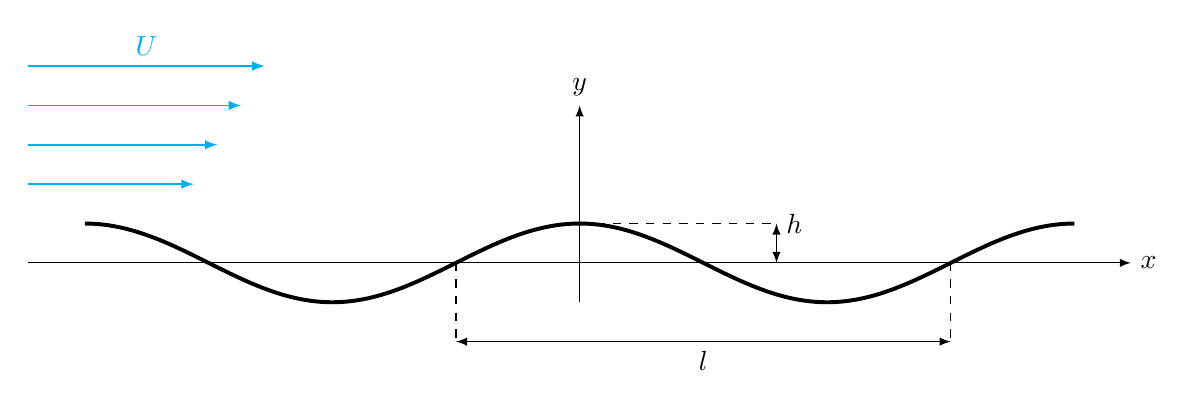
\begin{tikzpicture}[scale=1.0]
            % Achsen
        \def\startx{-7}
        \def\endx{-4}
        \def\starty{2.5}
        \def\ydis{0.5}
        \def\xenddis{0.3}
        \draw[->,>=latex] (-7, 0) -- (7, 0) node[right] {$x$};
        \draw[->,>=latex] (0, -0.5) -- (0, 2) node[above] {$y$};
        \draw[->,>=latex,cyan, line width=0.02cm] (\startx, \starty) -- (\endx, \starty) node[midway, yshift=0.25cm] {$U$};
        \draw[->,>=latex,cyan, line width=0.02cm] (\startx, \starty-\ydis) -- (\endx-\xenddis, \starty-\ydis);
        \draw[->,>=latex,cyan, line width=0.02cm] (\startx, \starty-2*\ydis) -- (\endx-2*\xenddis, \starty-2*\ydis);
        \draw[->,>=latex,cyan, line width=0.02cm] (\startx, \starty-3*\ydis) -- (\endx-3*\xenddis, \starty-3*\ydis);

        % % Gitterlinien optional
        % \draw[very thin, gray!30] (0, -1.5) grid[xstep=1, ystep=0.5] (7, 1.5);

        % Sinusfunktion
        \draw[thick, line width=0.05cm, black, domain=-2*pi:2*pi, samples=200] 
        plot (\x, {0.5*cos(\x r)});

        % Vermassungslinie l
        \def\xpos{0}
        \def\ypos{-1}
        \def\startmeas{-pi/2}
        \def\endmeas{3*pi/2}
        \draw[<->,>=latex] (\startmeas,\ypos) -- (\endmeas,\ypos) node[midway, below] {$l$};

        % Hilfslinien
        \draw[dashed] (\startmeas,\xpos) -- (\startmeas,\ypos);
        \draw[dashed] (\endmeas,\xpos) -- (\endmeas,\ypos);
        
        % Vermassungslinie h
        \def\xpos{2.5}
        \def\ypos{0}
        \def\startmeas{0}
        \def\endmeas{0.5}
        \draw[<->,>=latex] (\xpos,\startmeas) -- (\xpos,\endmeas) node[right] {$h$};

        % Hilfslinien
        \draw[dashed] (\startmeas,\endmeas) -- (\xpos,\endmeas);
        \draw[dashed] (\startmeas,\ypos) -- (\xpos,\ypos);
    \end{tikzpicture}
    }
    \caption{Strömung über einem Wellblech.
\index{Wellblech}}
    ~\label{fig:wellblech}
\end{figure}

% \end{document}

Dabei definieren wir das Potential als
\begin{align*}
    \Phi
    =
    U\,x + A\,\frac{l}{2\,\pi}\,\sin\left(\frac{2\,\pi\,x}{l}\right)
    \,e^{-\frac{2\,\pi\,y}{l}}
\end{align*}
wobei $U$ die ungestörte Geschwindigkeit im 
Unendlichen $y\rightarrow\infty$ bedeutet.

\subsection{Inkompressible Strömung}
Bei inkompressibler Strömung ist die
Laplace-Gleichung~\eqref{eq:laplace} sofort erfüllt.
Das kann bewiesen werden, indem wir für das Potential
die zweiten Ableitungen
\begin{align*}
    \frac{\partial\,^2\,\Phi}{\partial\,x^2}
    &= \frac{A\,2\,\pi}{l}\,\sin\left(\frac{2\,\pi\,x}{l}\right)
    e^{-\frac{2\,\pi\,y}{l}} \\
    \frac{\partial\,^2\,\Phi}{\partial\,y^2}
    &= -\frac{A\,2\,\pi}{l}\,\sin\left(\frac{2\,\pi\,x}{l}\right)
    \,e^{-\frac{2\,\pi\,y}{l}}
\end{align*}
berechnen wobei ersichtlich ist, dass
\begin{align*}
    \frac{\partial\,^2\,\Phi}{\partial\,x^2}
    =
    -\frac{\partial\,^2\,\Phi}{\partial\,y^2}.
\end{align*}
Es existiert dann auch eine sogenannte Stromfunktion
\begin{align*}
    \Psi
    =
    U\,y - A\,\frac{l}{2\,\pi}\,\cos\left(\frac{2\,\pi\,x}{l}\right)
    \,e^{-\frac{2\,\pi\,y}{l}},
\end{align*}
welche die Bedingung
\begin{align*}
    u 
    &=
    \frac{\partial\,\Phi}{\partial\,x}
    =
    \frac{\partial\,\Psi}{\partial\,y}
    \\
    v
    &=
    \frac{\partial\,\Phi}{\partial\,y}
    =
    -\frac{\partial\,\Psi}{\partial\,x}
\end{align*}
erfüllt.
Auch die Stromfunktion ist eine Lösung der Laplace-Gleichung
\begin{align*}
    \frac{\partial\,^2\,\Psi}{\partial\,x\,^2}
    +
    \frac{\partial\,^2\,\Psi}{\partial\,y\,^2}
    =
    0.
\end{align*}
Wenn wir $\Psi = 0$ setzen, dann erhalten wir die Gleichung
einer Stromlinie
\begin{align}
    0 = U\,y - A\,\frac{l}{2\,\pi}\,
    \cos\left(\frac{2\,\pi\,x}{l}\right)\,
    e^{-\frac{2\,\pi\,y}{l}},\label{eq:stromlinie}
\end{align}
aufgelöst nach $y$ ergibt das
\begin{align*}
    y
    =
    \frac{A}{U}\,\frac{l}{2\,pi}\,
    \cos\left(\frac{2\,\pi\,x}{l}\right)\,
    e^{-\frac{2\,\pi\,y}{l}}.
\end{align*}
Wir setzen zusätzlich 
\begin{align*}
    \frac{A}{U} \ll 1,
\end{align*}
damit näherungsweise gilt
\begin{align*}
    y
    =
    h\,\cos\left(\frac{2\,\pi\,x}{l}\right).
\end{align*}
Die Stromlinie sehr nahe am Wellblech ist eine
Kosinunslinie bzw. sie entspricht gerade der Kontur
des Blechs.
Die anderen Stromlinien $y > 0$ gehen mit zunehmendem $y$
in Gerade über, weil
\begin{align*}
    \lim_{y\,\to\,\infty}
    e^{-\frac{2\,\pi\,y}{l}}
    =
    0.
\end{align*}
Das Ganze sieht man auch in Abbildung~\ref{fig:stromlinien}.
\begin{figure}
    \centering
    \includegraphics[width=\textwidth]{papers/ueberschall/figures/Stromlinien.pdf}
    \caption{Stromlinien über dem Wellblech für $\frac{A}{U}=0.2$.}
    ~\label{fig:stromlinien}  
\end{figure}

Mit Hilfe der bernoullischen Gleichung, gemäss~\cite{BernoulliWikiDE},
\begin{align*}
    p_{\text{tot}} 
    = 
    p 
    + 
    \frac{1}{2}\,\rho\,V^2 
    + 
    \rho\,g\,z = \text{const},
\end{align*}
wobei $p_{\text{tot}}$ der Totaldruck ist, 
$\rho$ die Dichte des Fluids, $g$ die Erdbeschleunigung,
$V$ die Geschwindigkeit an einem Ort auf der Stromlinie 
und $z$ die Höhe über einem Bezugspunkt,
falls es sich um ein dreidimensionales Strömungsfeld handelt.

Da wir jedoch ausschliesslich in der $x,y$-Ebene arbeiten, 
fällt der letzte Term weg, weil $z = 0$.
Es bleibt somit:
\begin{align*}
    \underbrace{p}_{\text{statischer Druck}} 
    + 
    \underbrace{\frac{1}{2}\,\rho\,V^2}_{\text{dynamischer Druck}} 
    = 
    \text{const},
\end{align*}
was bedeutet, dass entlang einer Stromlinie 
der statische Druck und der dynamische Druck
zusammen konstant bleiben.

Wenn wir nun den lokalen Druck $p$ berechnen möchten, 
verwenden wir die freie Strömungsgeschwindigkeit $U$
als Referenzgrösse. 
Daraus ergibt sich:
\begin{align*}
    p_\infty 
    + 
    \frac{1}{2}\,\rho\,U^2 
    = 
    p 
    + 
    \frac{1}{2}\,\rho\,V^2,
\end{align*}
umgestellt nach dem lokalen Druck:
\begin{align*}
    p = p_\infty + \frac{1}{2}\,\rho\,(U^2 - V^2),
\end{align*}
wobei $V^2$ sich ergibt aus:
\begin{align*}
    V^2 = u^2 + v^2.
\end{align*}

Damit kann nun die Druckverteilung über dem Wellblech visualisiert werden, 
wie in Abbildung~\ref{fig:druckverteilung} dargestellt. 
Es handelt sich dabei um den relativen Druck, 
das heisst, der Druck ist bezogen auf den Umgebungsdruck. 
Deutlich erkennbar ist, dass der höchste Druck an den konkaven Stellen auftritt, 
während an den konvexen Stellen der niedrigste Druck herrscht.
\begin{figure}
    \centering
    \includegraphics[width=\textwidth]{papers/ueberschall/figures/Druckverteilung.pdf}
    \caption{Relative Druckverteilung über dem Wellblech.}
    ~\label{fig:druckverteilung}  
\end{figure}

\subsection{Kompressible Strömung}
Bei kompressibler Strömung gestaltet sich die Situation etwas komplexer.
Die Ausgangslage ist eine partielle Differentialgleichung zweiter Ordnung,
die durch geeignete Vereinfachungen auf jene Terme reduziert wurde, 
welche den grössten Einfluss auf die Abweichung haben.
Das genaue Vorgehen ist in~\cite{Ackeret1928} ausführlich dokumentiert.

Die folgende Gleichung stellt daher eine Näherungslösung dar,
die jedoch wesentliche Eigenschaften der exakten Lösung widerspiegelt:
\begin{align}
    \frac{\partial\,^2\,\Phi}{\partial\,x\,^2}\,
    \left(1-\frac{U^2}{a^2}\right)
    +
    \frac{\partial\,^2\,\Phi}{\partial\,y\,^2}
    =
    0\label{eq:kompressible_stroemung}
\end{align}
Der Ausdruck in der Klammer ist eine Konstante, d.h.
durch die einfache Koordinatentransformation
\begin{align*}
    x 
    &=
    \xi \\
    y\,\beta
    &=
    \eta \\
    \beta
    &=
    \sqrt{1-\frac{U^2}{a^2}}
\end{align*}
wird daraus wenig überraschend
\begin{align*}
    \frac{\partial\,^2\,\Phi}{\partial\,\xi\,^2}\,
    +
    \frac{\partial\,^2\,\Phi}{\partial\,\eta\,^2}
    =
    0
\end{align*}
die gewöhnlichen laplaceschen Gleichung, wie
bei der Potentialströmung.
Das Potential dieser kompressiblen Strömung ergibt sich zu
\begin{align*}
    \Phi
    =
    U\,x + A\,\frac{l}{2\,\pi}\,\sin\left(\frac{2\,\pi\,x}{l}\right)
    \,e^{-\frac{2\,\pi\,y\,\beta}{l}}
\end{align*}
und die dazugehörige Stromfunktion
\begin{align*}
    \Psi
    =
    U\,y - U\,\frac{h}{\beta^2}\,\cos\left(\frac{2\pi x}{l}\right)
    \,e^{-\frac{2\pi y \beta}{l}}.
\end{align*}
Durch gleiches Vorgehen wie bei Gleichung~\eqref{eq:stromlinie}
erhalten wir für $y\,\to\,0$
\begin{align*}
    y
    =
    \frac{A\,\beta\,l}{2\,\pi\,U}\,
    \cos\left(\frac{2\,\pi\,x}{l}\right).
\end{align*}
Damit wäre für kleine $y$ die Amplitude $h$ der Kosinuslinie
\begin{align*}
    h
    =
    \frac{A\,l\,\beta}{2\,\pi\,U}
\end{align*}
und somit 
\begin{align*}
    A
    =
    \frac{2\,\pi\,h\,U}{\beta\,l}.
\end{align*}
Demnach formulieren wir neu $\Phi$ als
\begin{align*}
    \Phi
    =
    U\,x + U\,\frac{h}{\beta}\,\sin\left(\frac{2\,\pi\,x}{l}\right)
    \,e^{-\frac{2\,\pi\,y\,\beta}{l}}.
\end{align*}
Der Faktor~$\beta$ beeinflusst das Abklingen der Störung,
wie in Abbildung~\ref{fig:abklingen_stromlinie} 
für drei verschiedene Fälle dargestellt ist.
Dazu werden die Stromlinien über einem Buckel visualisiert.
\begin{figure}
    \centering
    \begin{minipage}[b]{0.32\textwidth}
        \centering
        \includegraphics[width=\linewidth]{papers/ueberschall/figures/abklingen_10.pdf}
        \caption*{$\beta = 1$ ; $U = 10\,\frac{\mathrm{m}}{\mathrm{s}}$}
    \end{minipage}
    \hfill
    \begin{minipage}[b]{0.32\textwidth}
        \centering
        \includegraphics[width=\linewidth]{papers/ueberschall/figures/abklingen_200.pdf}
        \caption*{$\beta = 0.81$ ; $U = 200\,\frac{\mathrm{m}}{\mathrm{s}}$}
    \end{minipage}
    \hfill
    \begin{minipage}[b]{0.32\textwidth}
        \centering
        \includegraphics[width=\linewidth]{papers/ueberschall/figures/abklingen_340.pdf}
        \caption*{$\beta = 0$ ; $U = a$}
    \end{minipage}
    \caption{Stromlinien bei verschiedenen Strömungsgeschwindigkeiten im Unterschall.}
~\label{fig:abklingen_stromlinie}
\end{figure}

\subsection{Überschall}
Nun betrachten wir die Strömung im Überschallbereich.
Wir starten dabei bereits mit der vereinfachten 
Gleichung~\eqref{eq:kompressible_stroemung}:
\begin{align*}
    \frac{\partial^2\,\Phi}{\partial\,x^2}
    \left(1 - \frac{U^2}{a^2}\right)
    =
    -\frac{\partial^2\,\Phi}{\partial\,y^2},
\end{align*}
wobei der rechte Term zur besseren Übersicht auf die 
linke Seite verschoben wurde.

Da im Überschallbereich $U > a$ gilt, wird der Ausdruck 
in der Klammer negativ.
Es ist daher sinnvoll, die Gleichung in folgender 
Form umzuschreiben:
\begin{align*}
    \frac{\partial^2\,\Phi}{\partial\,x^2}
    \left(\frac{U^2}{a^2} - 1\right)
    =
    \frac{\partial^2\,\Phi}{\partial\,y^2}.
\end{align*}

Führen wir nun eine geeignete Koordinatentransformation durch,
\begin{align*}
    x 
    &= 
    \xi, \\
    y\,\beta 
    &= 
    \eta,
\end{align*}
mit dem Parameter
\begin{align*}
    \beta = \sqrt{\frac{U^2}{a^2} - 1},
\end{align*}
so ergibt sich die transformierte Gleichung:
\begin{align*}
    \frac{\partial^2\,\Phi}{\partial\,\xi^2}
    -
    \frac{\partial^2\,\Phi}{\partial\,\eta^2}
    =
    0.
\end{align*}
Diese Gleichung ähnelt formal der ursprünglichen Gleichung 
für den Unterschallbereich, weist jedoch ein 
unterschiedliches Vorzeichen im zweiten Term auf.
Dementsprechend handelt es sich hier um eine hyperbolische 
Differentialgleichung, die Wellenvorgänge beschreibt.
Das Strömungsverhalten im Überschallbereich ist daher — 
in gewisser Weise — mit dem Verhalten von Wellen in Wasser vergleichbar.

%
% teil3.tex -- Beispiel-File für Teil 3
%
% (c) 2020 Prof Dr Andreas Müller, Hochschule Rapperswil
%
% !TEX root = ../../buch.tex
% !TEX encoding = UTF-8
%
\section{Teil 3
\label{ueberschall:section:teil3}}
\kopfrechts{Teil 3}

Wir beginnen hier mit der homogenen Wellengleichung
\begin{equation}
    \frac{\partial^2u}{\partial t^2}
    =
    \frac{\partial^2u}{\partial x^2} +
    \frac{\partial^2u}{\partial y^2} +
    \frac{\partial^2u}{\partial z^2},\\
\label{ueberschall:wellengleichung}
\end{equation}
welches eine lineare partielle Differentialgleichung zweiter Ordnung ist
für eine relle Funktion $u(t,x,y,z)$ des dreidimensionalen Raumes und der Zeit.

\subsection{De finibus bonorum et malorum
\label{ueberschall:subsection:malorum}}
test

\printbibliography[heading=subbibliography]
\end{refsection}
